\documentclass[tikz,border=3.14mm]{standalone}
\begin{document}
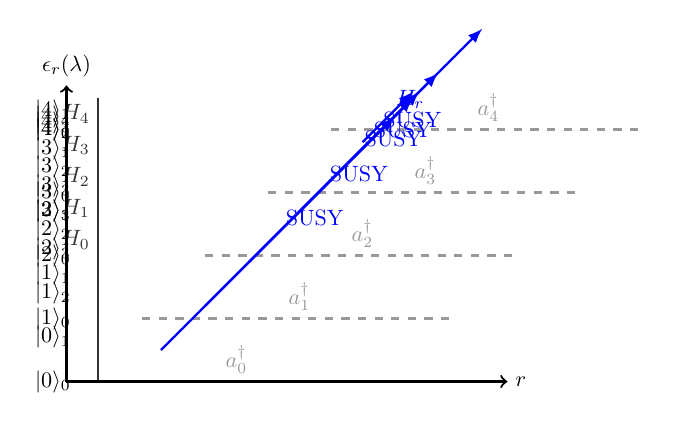
\begin{tikzpicture}[thick,scale=0.8, every node/.style={scale=0.8}]
    % Draw vertical lines (energy levels)
    \draw[black!80] (-1,0) -- ++(0,4.5) node[midway,left] {$H_0$};
    \draw[black!80] (-1,1) -- ++(0,3.5) node[midway,left] {$H_1$};
    \draw[black!80] (-1,2) -- ++(0,2.5) node[midway,left] {$H_2$};
    \draw[black!80] (-1,3) -- ++(0,1.5) node[midway,left] {$H_3$};
    \draw[black!80] (-1,4) -- ++(0,0.5) node[midway,left] {$H_4$};
    
    % Draw horizontal lines (states)
    \node at (-1.3,0) [left] {$|0\rangle_0$};
    \node at (-1.3,1) [left] {$|1\rangle_0$};
    \node at (-1.3,2) [left] {$|2\rangle_0$};
    \node at (-1.3,3) [left] {$|3\rangle_0$};
    \node at (-1.3,4) [left] {$|4\rangle_0$};
    
    \node at (-1.3,0.7) [left] {$|0\rangle_1$};
    \node at (-1.3,1.7) [left] {$|1\rangle_1$};
    \node at (-1.3,2.7) [left] {$|2\rangle_1$};
    \node at (-1.3,3.7) [left] {$|3\rangle_1$};
    \node at (-1.3,4.3) [left] {$|4\rangle_1$};
    
    \node at (-1.3,1.4) [left] {$|1\rangle_2$};
    \node at (-1.3,2.4) [left] {$|2\rangle_2$};
    \node at (-1.3,3.4) [left] {$|3\rangle_2$};
    \node at (-1.3,4.0) [left] {$|4\rangle_2$};
    
    \node at (-1.3,2.1) [left] {$|2\rangle_3$};
    \node at (-1.3,3.1) [left] {$|3\rangle_3$};
    \node at (-1.3,4.1) [left] {$|4\rangle_3$};
    
    \node at (-1.3,2.7) [left] {$|3\rangle_3$};
    \node at (-1.3,4.2) [left] {$|4\rangle_4$};
    
    % Create dashed lines for factorization operators
    \foreach \i in {0,1,2,3,4}
    {
        \draw[dashed, black!40] (\i-1.3, \i) -- ++(5,0) node[midway, above] {$a^\dagger_{\i}$};
    }
    
    % Draw the diagonal lines with "SUSY" labels
    \draw[blue,-latex] (0,0.5) -- ++(3.7,3.7) node [midway, above right] {SUSY};
    \draw[blue,-latex] (0.7,1.2) -- ++(3.7,3.7) node [midway, above right] {SUSY};
    \draw[blue,-latex] (1.4,1.9) -- ++(3.7,3.7) node [midway, above right] {SUSY};
    \draw[blue,-latex] (2.1,2.6) -- ++(2,2) node [midway, above right] {SUSY};
    \draw[blue,-latex] (2.8,3.3) -- ++(1.2,1.2) node [midway, above right] {SUSY};
    \draw[blue,-latex] (3.2,3.8) -- ++(0.8,0.8) node [midway, above right] {$H_r$};
    
    % Draw the horizontal axis
    \draw[->] (-1.5,0) -- (5.5,0) node[right] {$r$};
    
    % Draw the vertical axis
    \draw[->] (-1.5,0) -- (-1.5,4.7) node[above] {$\epsilon_r(\lambda)$};
    
\end{tikzpicture}
\end{document}